We consider static data structures which makes modifications to the data structures infeasible.

The algorithms we have focused on is classic binary search (in-order layout), binary tree (BFS), binary tree (DFS) and a blocked tree with BFS and DFS layout. All data structures are stored in single arrays.

For tree structures we always construct complete trees. In case the amount of data does not fill the tree, dummy data are used. The dummy data are MAX\_INT's. We never query MAX\_INT so we do not touch the dumma data. Thus the performance of the queries should not be affected.

For each of the algorithms we theoretically analyzed the number of branch predictions and cache faults. The binary algorithms all have 50\% chance of a branch misprediction at each level and analysis of those are therefore omitted. We made the assumption that the cache is hot because we use a large number of queries in each test.

In the following sections we use these definitions:
\begin{eqnarray*}
\begin{array}{rcl}
n & : & \textrm{Number of 32 bit ints} \\
B & : & \textrm{Size of cacheline (in 32 bit ints)} \\
M & : & \textrm{Size of cache (in 32 bit ints)}
\end{array}
\end{eqnarray*}

\subsection{Binary search}

Contrary to the tree algorithms the binary search does not require any dummy data to be inserted.

\subsubsection*{Expected cache faults}

% TODO: Er -log2 B korrekt? Nok naermere 1/2 af det? Taenker man stadig kan hoppe udenfor?

\begin{eqnarray*}
\log_2 n - \log_2 B - \log_2 \frac{M}{B} 
\end{eqnarray*}
where $\log_2 B$ is the bottom where we make small jumps. The first elements we visit is far from each other so we need a whole cacheline for each. $\log_2 \frac{M}{B}$ is the "top" $\frac{M}{B}$ cachelines.

\subsection{Binary BFS layout}

...

\begin{eqnarray*}
\mathrm{left}(i) & = & 2i \\
\mathrm{right}(i) & = & 2i + 1
\end{eqnarray*}

\subsubsection*{Expected cache faults}

\begin{eqnarray*}
\log_2 n - \log_2 M 
\end{eqnarray*}
where $\log_2 M$ is the top of the tree.

\subsection{Binary DFS layout}

...

\begin{eqnarray*}
|L| & : & \textrm{Number of elements in left subtree} \\
\\
\mathrm{left}(i) & = & i + 1 \\
\mathrm{right}(i) & = & i + |L| + 1
\end{eqnarray*}

\subsubsection*{Expected cache faults}

\begin{eqnarray*}
(\frac{1}{2}\frac{1}{B} + \frac{1}{2})\log_2 n - \log_2 B - \log_2 M 
\end{eqnarray*}
where $\log_2 M$ is the top of the tree. $\log_2 B$ is the last few levels where $|L|$ gets small enough such that a subtree is smaller than a cacheline. $\frac{1}{2}\frac{1}{B}$ is when we go left and $\frac{1}{2}$ is when we go right.

\subsection{Blocked BFS layout}

The blocked BFS layout contains $d - 1$ elements per node/leaf where $d$ is the arity of the tree. These blocks are laid in a breadth-first layout.

\begin{eqnarray*}
d & : & \textrm{Arity of the tree} \\
j & : & \textrm{Element in block $i$ (leftmost: $0$)} \\
\\
\mathrm{element}(i, j) & = & d\cdot (i - 1) + j + 1
\end{eqnarray*}

\subsubsection*{Scanning}

Internally in the nodes we employed two different ways to scan through the elements. Linear scan and binary search.

\subsubsection*{Expected cache faults, linear scan}

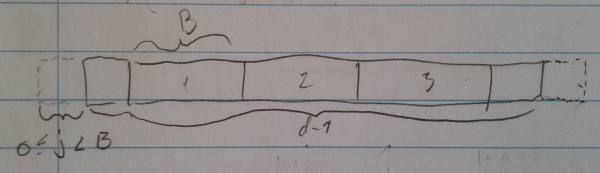
\includegraphics[width=1\textwidth]{blocks}
% TODO: Numre paa cachelines

We have defined the following stochastic variables:
\begin{eqnarray*}
X & : & \textrm{Number of cachelines we visit}\\
S & : & \textrm{A block's location from a cacheline boundary}
\end{eqnarray*}
The expected number of cache faults for each level is
\begin{eqnarray*}
E(X) = \sum_{i=1}^{m}i\cdot P(X=i)
\end{eqnarray*}
which is sum of the probabilities that we visit $i$ cachelines multiplied by $i$k were, where $m$ is the highest number of cachelines a block overlaps with.
\begin{eqnarray*}
m = \left\lfloor \frac{d-1-2}{B}\right\rfloor + 2
\end{eqnarray*}
With the law of total probability, the probability that we visit $i$ cachelines can be written as the sum of the probabilities that we end up in $i$ given a certain skew multiplied by the probability of the skew.
\begin{eqnarray*}
P(X=i) = \sum_{j=0}^{B-1}P(X=i\,|\, S=j)P(S=j)
\end{eqnarray*}
In the following calculations we have assumed an uniform distribution of where the linear scan stops in the block. If $d - 1 < B - j$ (i.e. the block does not lie on a cacheline boundary) then the probability of visiting a single cacheline is 1. Otherwise, it is the size of the block overlapping with the first possible cacheline divided by the size of the block. The probability of visiting a cacheline in the middle is just the size of a cacheline divided by the size of the block. For the last cacheline, the probability is the complement of the rest combined.
\begin{eqnarray*}
P(X=1\,|\, S=j) & = & \frac{\min\{B-j,\, d-1\}}{d-1}\\
\\
\underset{1 < i < m}{P(X=i\,|\, S=j)} & = & \frac{B}{d-1}\\
\\
\underset{m\neq1}{P(X=m\,|\, S=j)} & = & 1-\sum_{i=1}^{m-1}P(X=i\,|\, S=j)
\end{eqnarray*}
For the probability of starting with a skew $j$, we assumed an uniform distribution of the possible $j$'s and assumed the first block to be aligned with the cachelines. For example we have $P(S = 0) = P(S = 8) = \frac{1}{2}$ for $B = 16$, $d - 1 = 8$.
\begin{eqnarray*}
S_k & = & \{ 0 \leq x < B\ |\ x \in \mathbb{N} \wedge (d - 1)x\ \textrm{mod}\ B = k \}\\
\\
P(S=j) & = & \frac{|S_k|}{B}
\end{eqnarray*}

\paragraph*{Cache faults}

$\log_{d}\, n\cdot E(X)-\log_{d}\frac{M}{d-1}$

where $\log_{d}\, n\cdot E(X)$ is the number of cache faults per level. But because we assume the cache is hot, the top of the tree ($\log_{d}\frac{M}{d-1}$) is in cache.

\subsubsection*{Example, $B=16,\, M=2^{14},\, n=10^{6}$}

\begin{tabular}{|c|c|}
\hline 
$d$ & Expected cache faults\tabularnewline
\hline 
\hline 
2 & 5.59\tabularnewline
\hline 
5 & 3.42\tabularnewline
\hline 
9 & 2.82\tabularnewline
\hline 
16 & 4.64\tabularnewline
\hline 
17 & 2.43\tabularnewline
\hline 
18 & 4.793\tabularnewline
\hline 
33 & 4.14\tabularnewline
\hline 
\end{tabular}
\\
\\
As we can see from the examples we should expect fewest cache faults when the block size is equal to the cacheline size. Furthermore, we can see that if blocks are not aligned with cacheline boundaries then the amount of cache faults increases.

% TODO: Mispredictions

\subsection{Blocked DFS layout}

As with the blocked BFS layout, this layout contains $d - 1$ elements per node/leaf where $d$ is the arity of the tree. These blocks are laid in a depth-first layout.

\begin{eqnarray*}
d & : & \textrm{Arity of the tree} \\
j & : & \textrm{Element in block $i$ (leftmost: $0$)} \\
|S| & : & \textrm{Number of elements in a subtree} \\
\\
\mathrm{element}(i, j) & = & i + j\cdot |S| + 1
\end{eqnarray*}

% TODO: Cache faults + mispredictions